\chapter{Introdução Teórica}

\citeonline{Dias1994}  diz que a "Educação Ambiental se caracteriza por
incorporar as dimensões sociais, políticas, econômicas,
culturais, ecológicas e éticas, deixando claro que ao discutir
qualquer problema ambiental é fundamental a consideração
de todos estes aspectos." Segundo este autor, "a maior parte
dos problemas ambientais tem suas raízes na miséria que,
por sua vez, é gerada por políticas e problemas econômicos,
concentradores de riqueza e responsáveis pelo desemprego
e degradação ambiental."\\

Pode-se definir a educação ambiental, nas palavras de \citeonline{Magalhaes2018}, como um processo
onde o educando obtém conhecimentos acerca das
questões ambientais e assim passa a ter um novo
entendimento acerca do meio ambiente, se tornando um
agente transformador referente à preservação do meio
ambiente e de seus recursos naturais. \\

\citeonline{Gadotti2000} explica que educação ambiental vai muito além do conservacionismo
Trata-se de uma mudança radical de mentalidade em
relação à qualidade de vida, que está diretamente ligada
ao tipo de convivência que mantemos com a natureza e
que implica em atitudes, valores, ações. Trata-se de uma
opção de vida por uma relação saudável e equilibrada,
com o contexto, com os outros, com o ambiente mais
próximo, a começar pelo ambiente de trabalho e
doméstico.\\


Brasília foi inaugurada em 21 de abril de 1960

De acordo com o \citeonline{CODEPLANSEPLAN2013}

\begin{figure}[h]
    \centering
    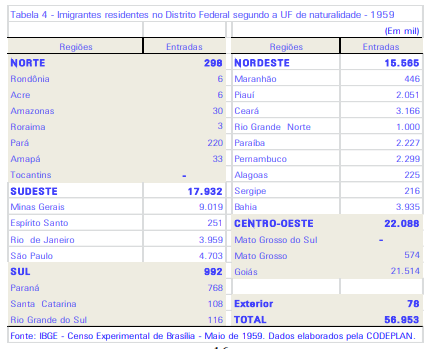
\includegraphics[width=0.7\linewidth]{fig/imigrantes-1959}
    \label{fig:imigrantes-1959}
    \caption{Imigrantes residentes no DF em 1959}
\end{figure}

\lipsum[1-30]

\begin{figure}[h]
    \centering
    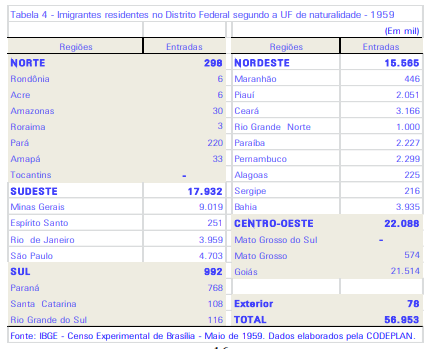
\includegraphics[width=0.7\linewidth]{fig/imigrantes-1959}
    \caption{}
%    \label{fig:imigrantes-1959}
\end{figure}

\begin{figure}[h]
    \centering
    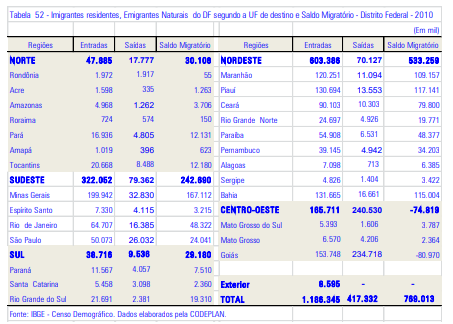
\includegraphics[width=0.7\linewidth]{fig/imigrantes-2010}
    \caption{}
    \label{fig:imigrantes-2010}
\end{figure}
